\begin{frame}
    \frametitle{ROLLO: Reactor evOLutionary aLgorithm Optimizer}
    \begin{itemize}
        \item ROLLO is a Python package that applies evolutionary algorithm
        techniques to optimize nuclear reactor design.
        \item ROLLO couples an evolutionary algorithm driver, Distributed 
        Evolutionary Algorithms in Python (DEAP), with 
        nuclear software, such as neutron transport OpenMC and thermal-hydraulics 
        Moltres codes.
    \end{itemize}
    \begin{block}{ROLLO Design Goals}
        \begin{itemize}
            \item Effective: good documentation, well tested, version controlled 
            on Github 
            \item Flexible: user can vary any imaginable parameter because
            ROLLO uses a templating method to edit the input file of the coupled software.
            \item Open-source: utilizes only open-source dependencies 
            \item Parallel: toggle to enable parallelization on local and HPCs
            \item Reproducible: Data from every ROLLO run saves into a unique, 
            pickled file (pickle is a Python module that serializes Python 
            objects), and all results from this work are available on Github.
        \end{itemize}
    \end{block}
\end{frame}

\begin{frame}
    \frametitle{ROLLO: Reactor evOLutionary aLgorithm Optimizer}
    \begin{figure}
        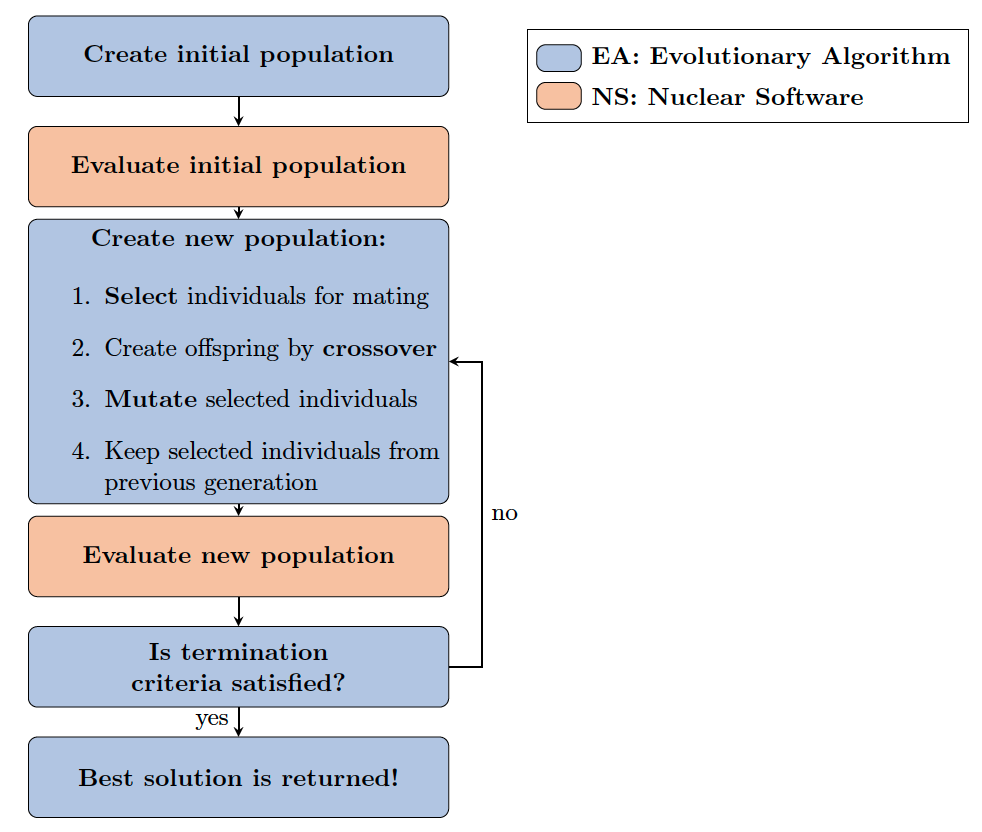
\includegraphics[width=0.8\linewidth]{figures/rollo-flow.png} 
        \caption{Process of finding optimal solutions for a problem with a 
        genetic algorithm. Nuclear software evaluates each new population.}
    \end{figure}
\end{frame}

\begin{frame}
    \frametitle{ROLLO Class Architecture}
    \begin{figure}
        \centering
        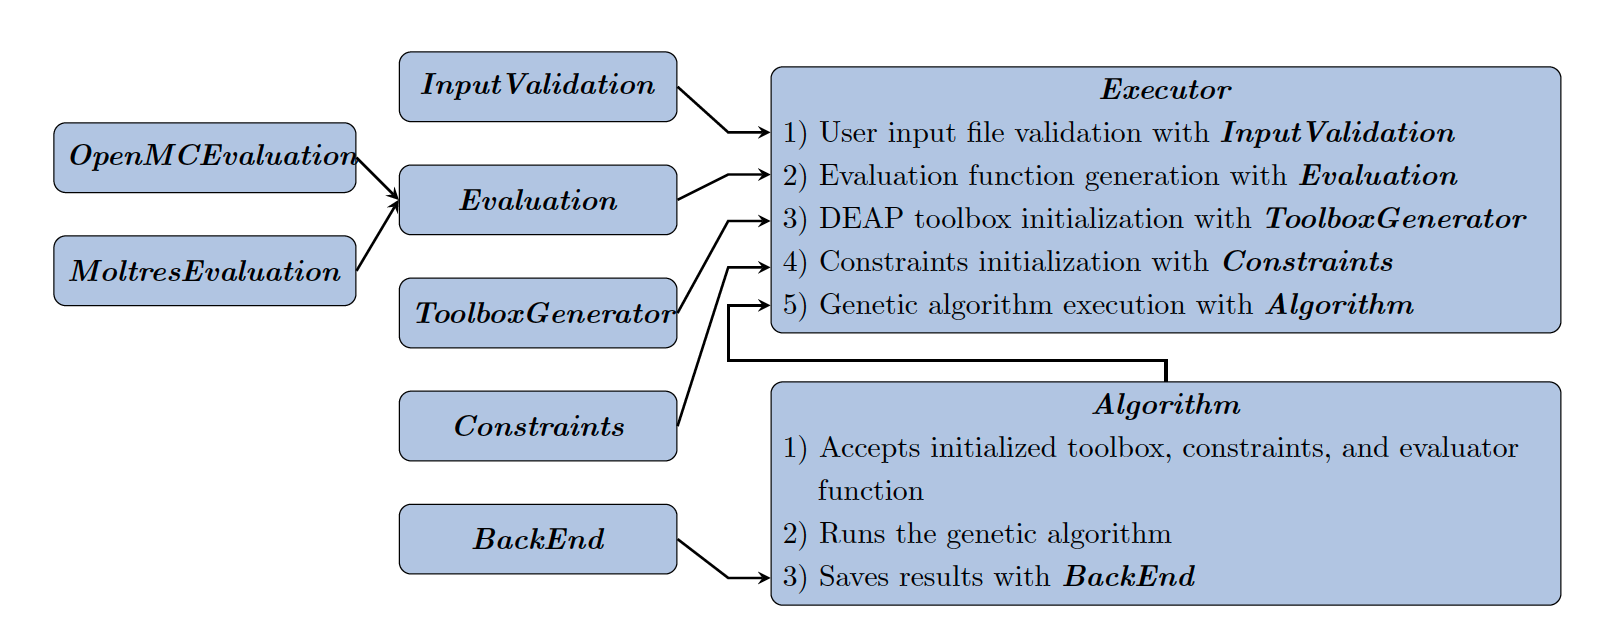
\includegraphics[width=1.1\linewidth]{figures/rollo-architecture.png} 
        \caption{Visualization of ROLLO architecture.}
    \end{figure}
\end{frame}